\monster{Chaos}{10}{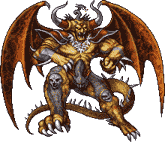
\includegraphics[width=0.23\textwidth]{./art/monsters/chaos.png}}
{
	HP: & \hfill 400 & MP: & \hfill 700 \\
	STR: & \hfill 8 & DEF: & \hfill 8 \\
	MAG: & \hfill 10 & RES: & \hfill 7 \\
	AGI: & \hfill 4 & Size: & \hfill L\\
}
{
	\textbf{Beam}: 5d DMG, 3u Range \hfill \textbf{Drops:} 10000 Gil \\
	\textbf{Immune}: \hyperlink{status}{All Status Effects} \\
	\textbf{Resilient}:\dark\fire
	
	\mspell{Ultima}{45}{3r}{3u}{5u}{
	You deal 10d+10 \hyperlink{type}{dark} damage only to enemies in the target area.  
	}{\dark}		
	\mspell{Curaja}{30}{2r}{3u}{5u}{
	All allies in the target area regain 8d+10 HP.  
	}{}	
	\mspell{Firaja}{28}{2r}{3u}{8u}{
	You deal 8d+10 \hyperlink{type}{fire} damage to everyone in the target area.
	}{\fire}
	\mpassive{Chaos Touch}{
		Whenever you successfully \hyperlink{action}{Attack} a target he makes a DC 8 check and suffers \hyperlink{status}{Poison}, \hyperlink{status}{Blind} and \hyperlink{status}{Silence} for 3 rounds upon failure.
	}
	\mreaction{Quicken}{
		Whenever you suffer damage, you can make a DC 6 check and if you succeed, take an additional turn after the attacker.
		This effect does not change the usual turn order and you can only use it once per round.
	}
	\vspace{0.1cm} \hrule \vspace{0.1cm} 
	"But I will be reborn once more. So even as you die, again and again, I shall return. Born again in this endless cycle I have created!" -- Chaos
}
